\begin{figure}[h]
	\centering
	\begin{minipage}{.5\textwidth}
		\capstart
		\centering
		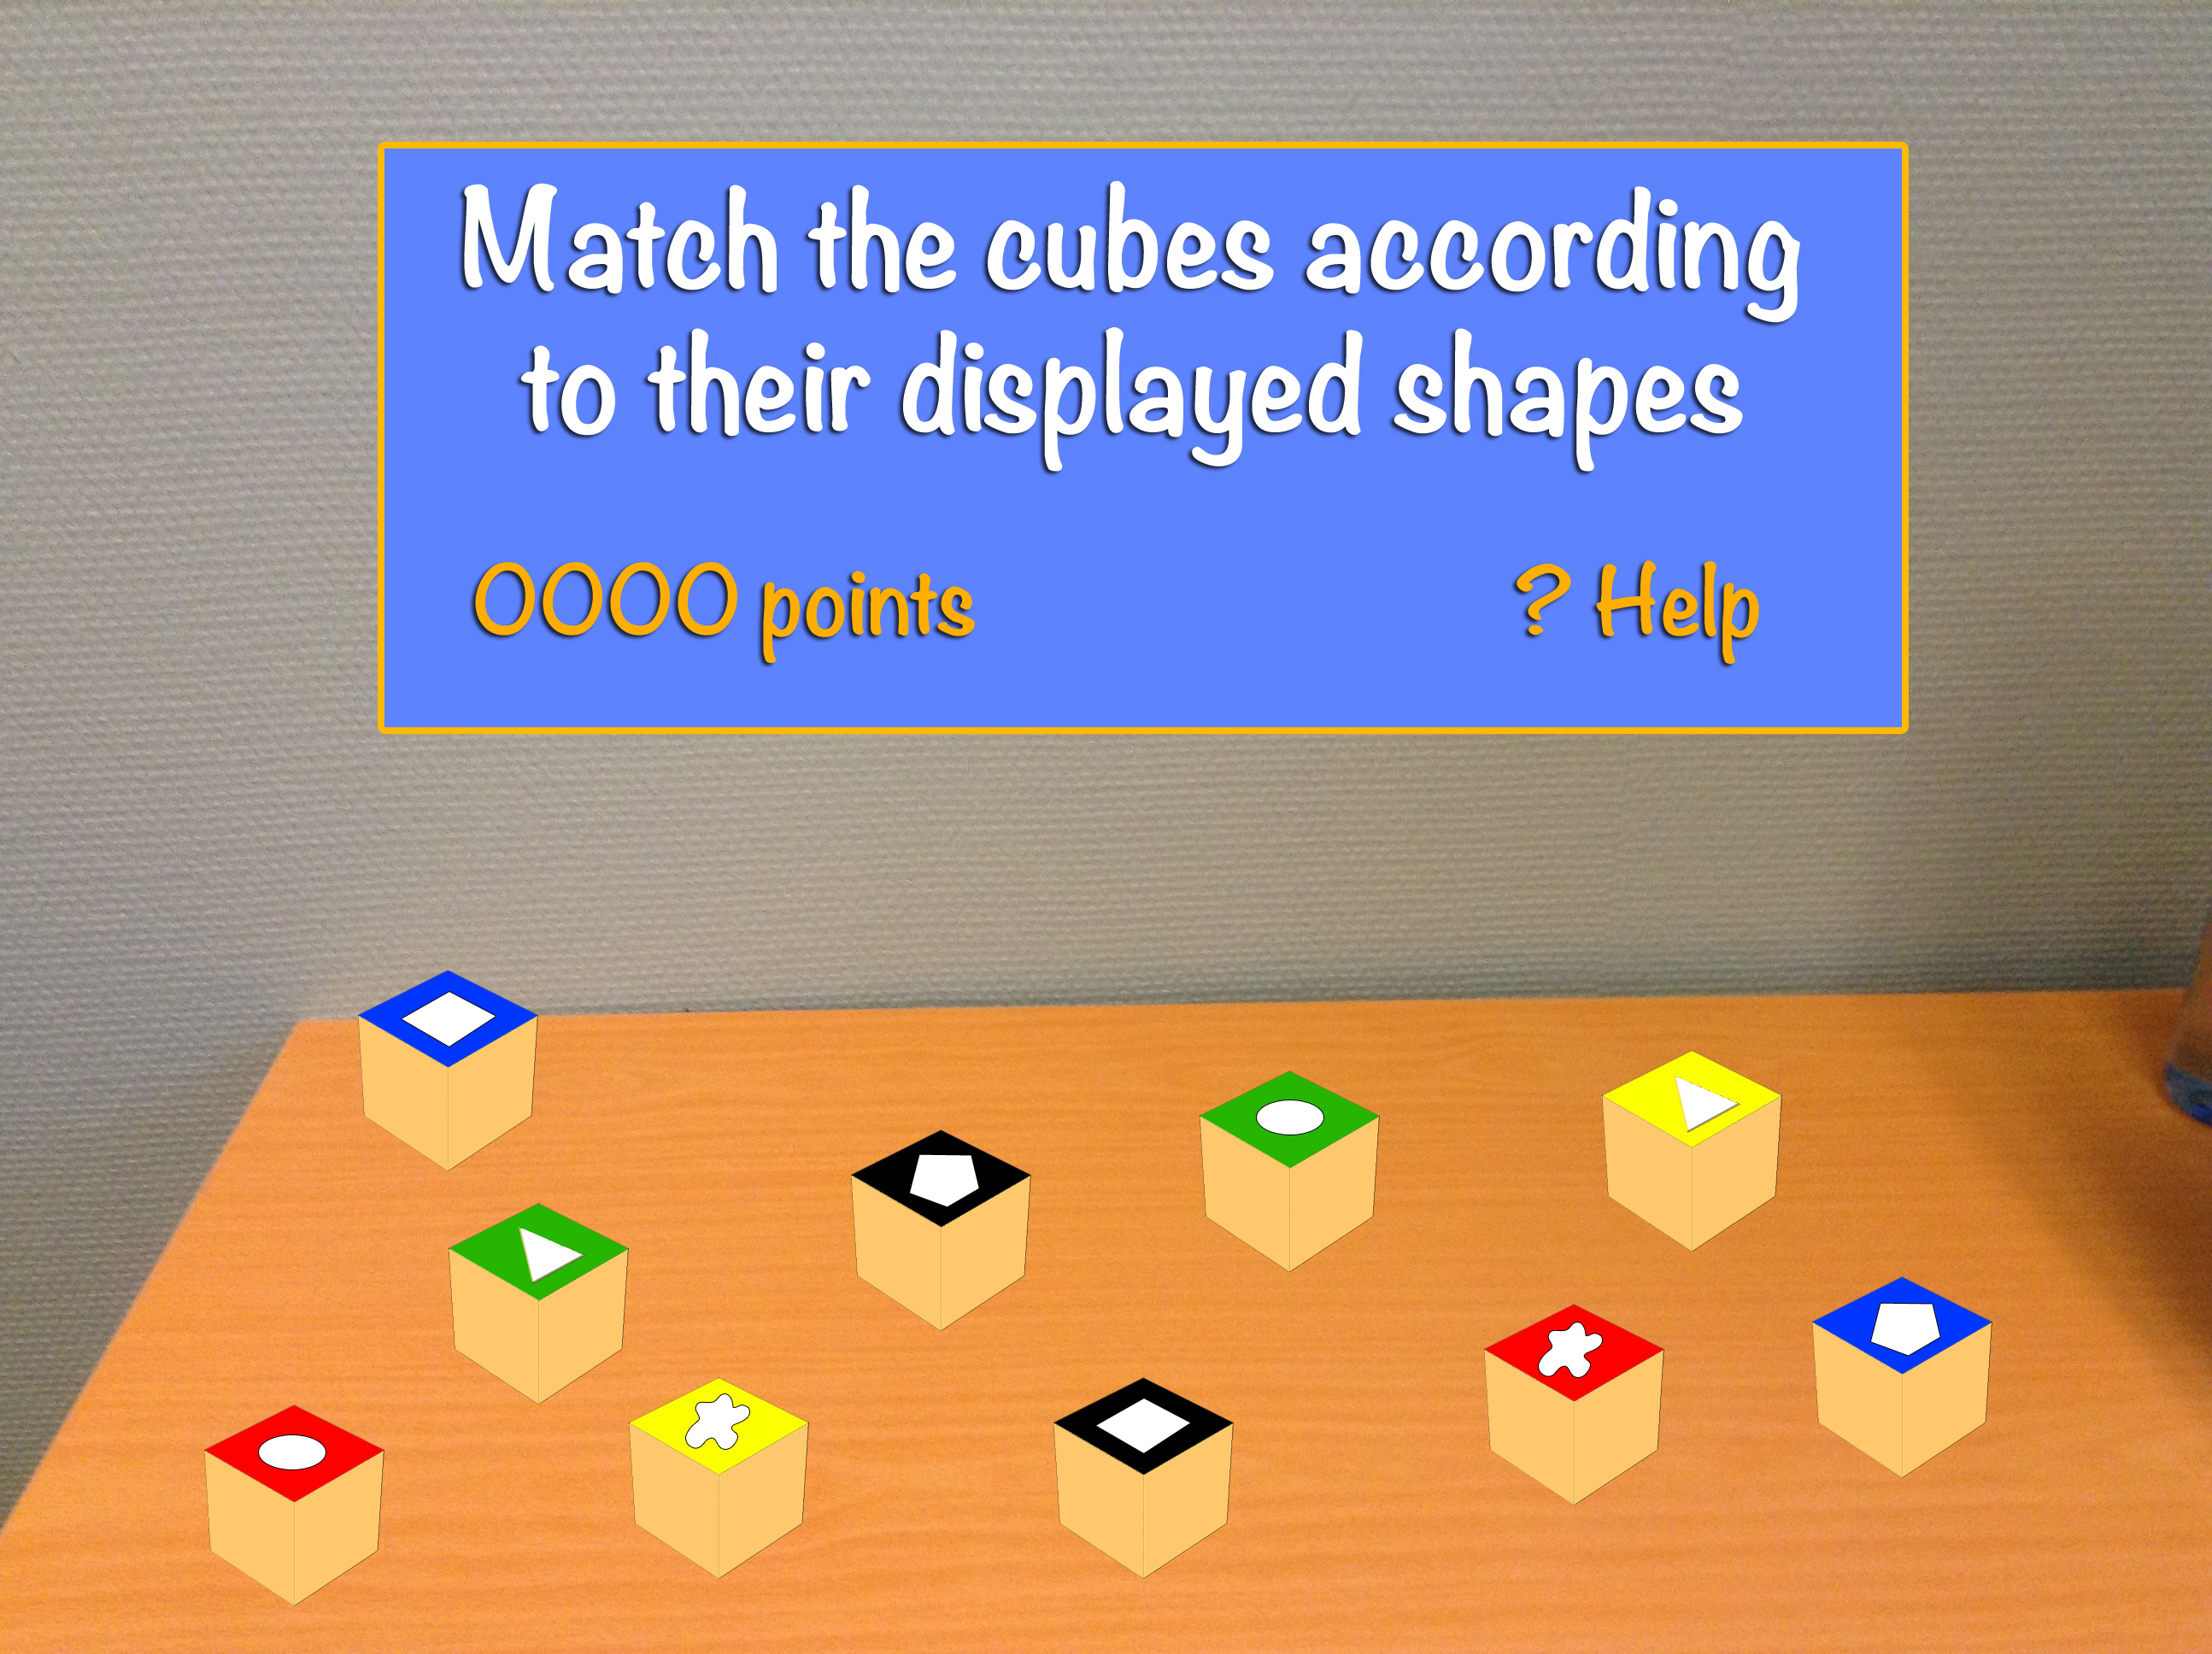
\includegraphics[width=0.9\textwidth]{images/Costas/game_mockup1(matching).jpg}
		\vspace{-10pt}
		\caption{Shape Match}
		\label{fig:Costas_shape_match}
	\end{minipage}%
	\begin{minipage}{.5\textwidth}
		\capstart
		\centering
		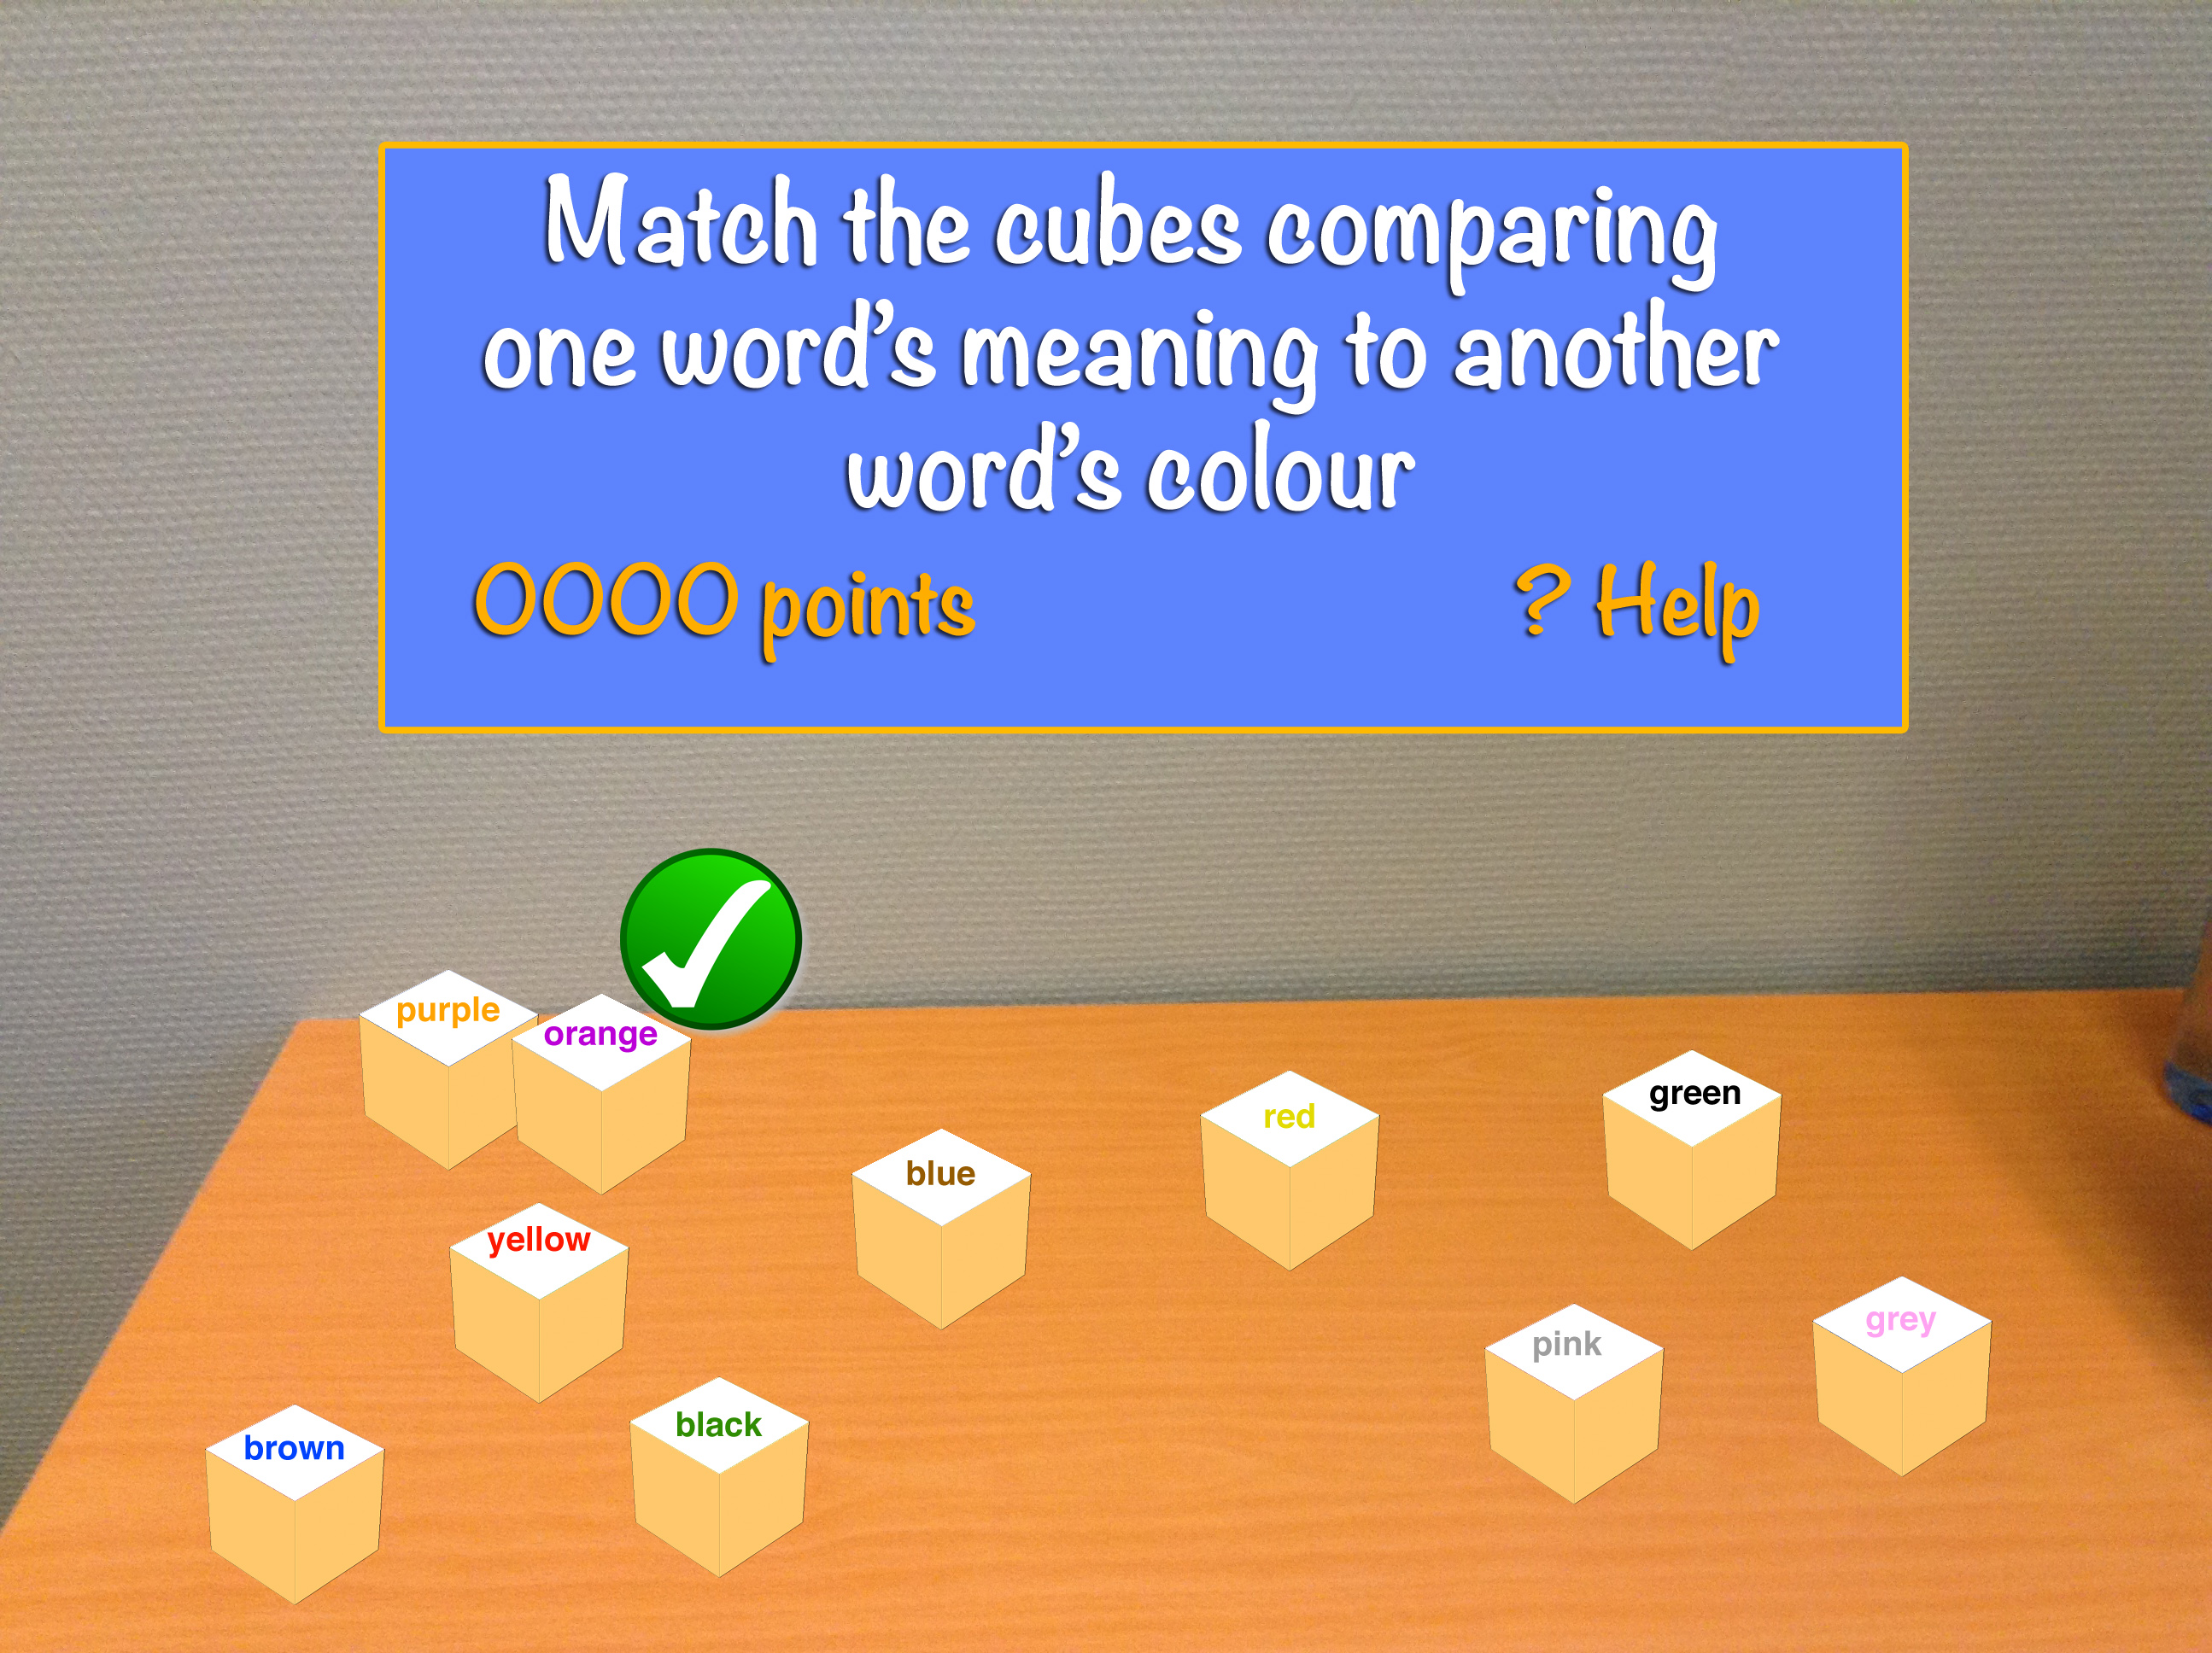
\includegraphics[width=0.9\textwidth]{images/Costas/game_mockup1(matching2).jpg}
		\vspace{-10pt}
		\caption{Colour Match}
		\label{fig:Costas_colour_match}
	\end{minipage}%
\end{figure}

\subsection{Shape Match}
	\label{game:shape_match} 

In this game the user combines pairs of cubes with matching patterns until all patterns have been found and put together.
The level is over either when all the pairs have been correctly placed together or time runs out.


\subsection{Colour Match}
	\label{game:colour_match}

This game also have users match up pairs of cubes, but instead of matching up figures and shapes the user have to pair up words and colours. For example one cube will have the text 'RED' written in a purple colour, and another box will have 'PURPLE' written in a red colour. The player have to pair up 10 cubes to a total of 5 pairs of such pairings.
The level is over either when all the pairs have been found or the time runs out.

\begin{figure}[h]
	\capstart
	\centering
	\begin{minipage}{.5\textwidth}
		\capstart
		\centering
		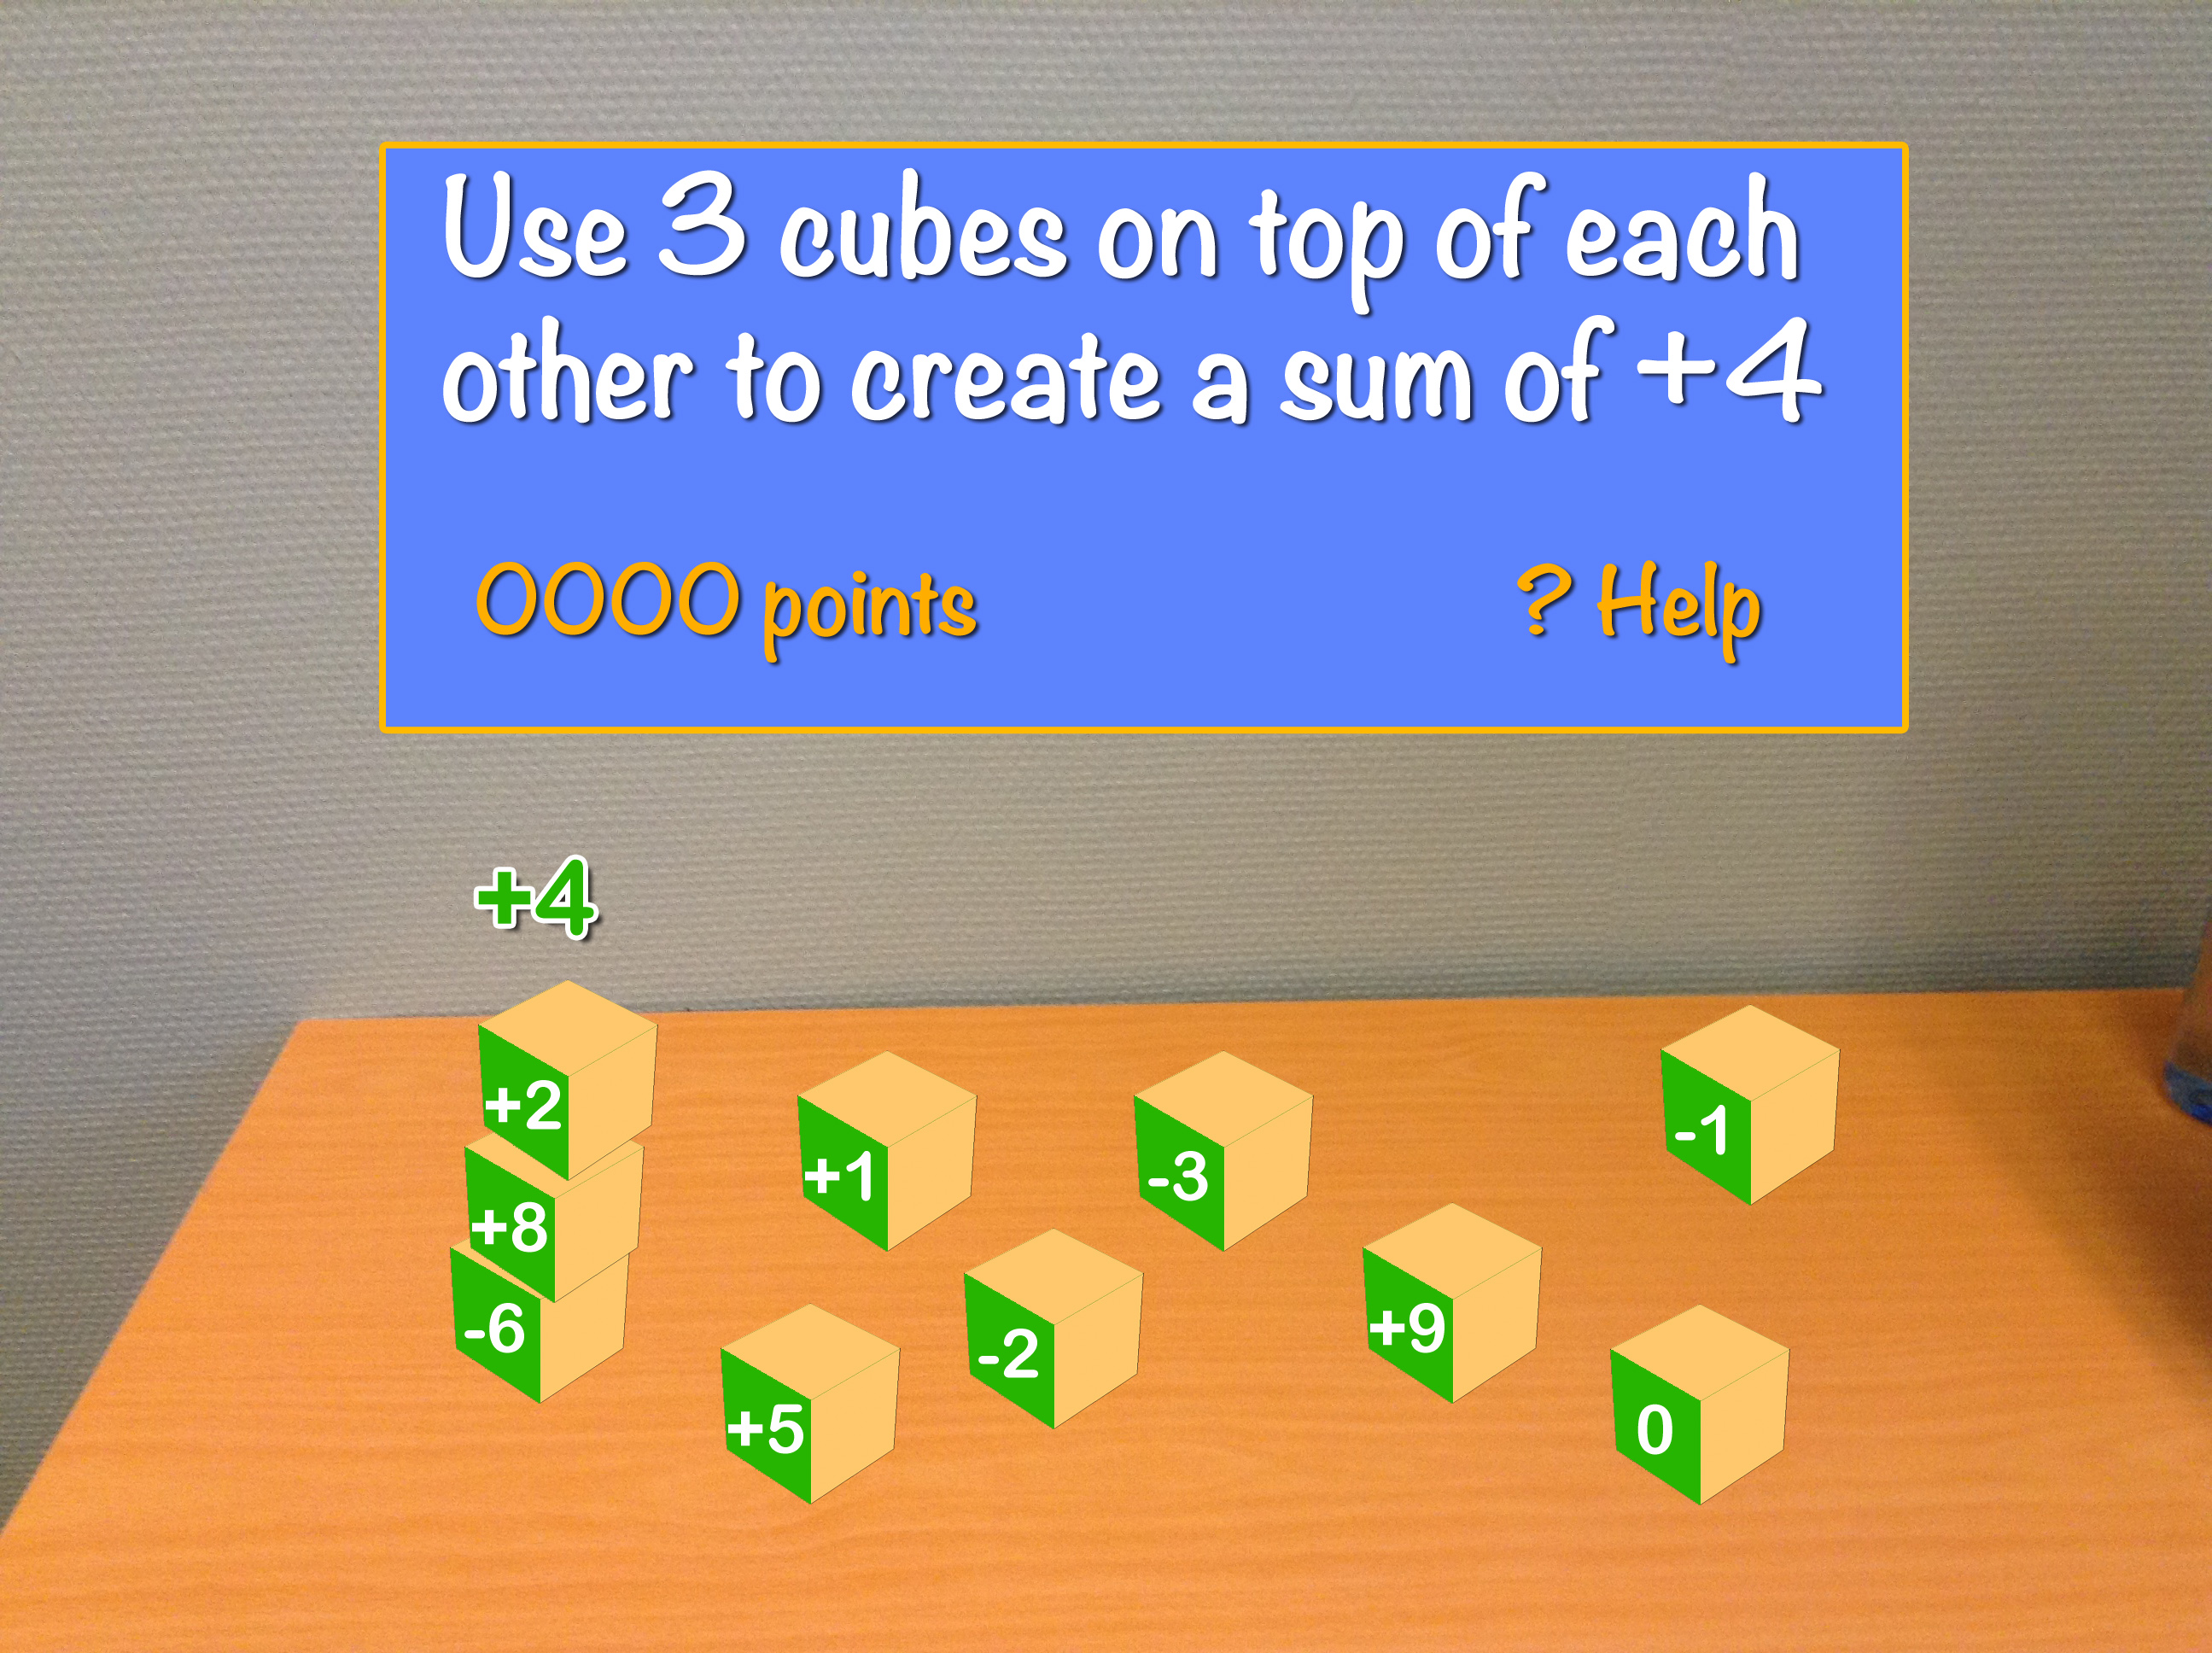
\includegraphics[width=0.9\textwidth]{images/Costas/game_mockup2(arithmetic).jpg}
		\vspace{-10pt}
		\caption{Total Sum}
		\label{fig:Costas_total_sum}
	\end{minipage}%
	\begin{minipage}{.5\textwidth}
		\capstart
		\centering
		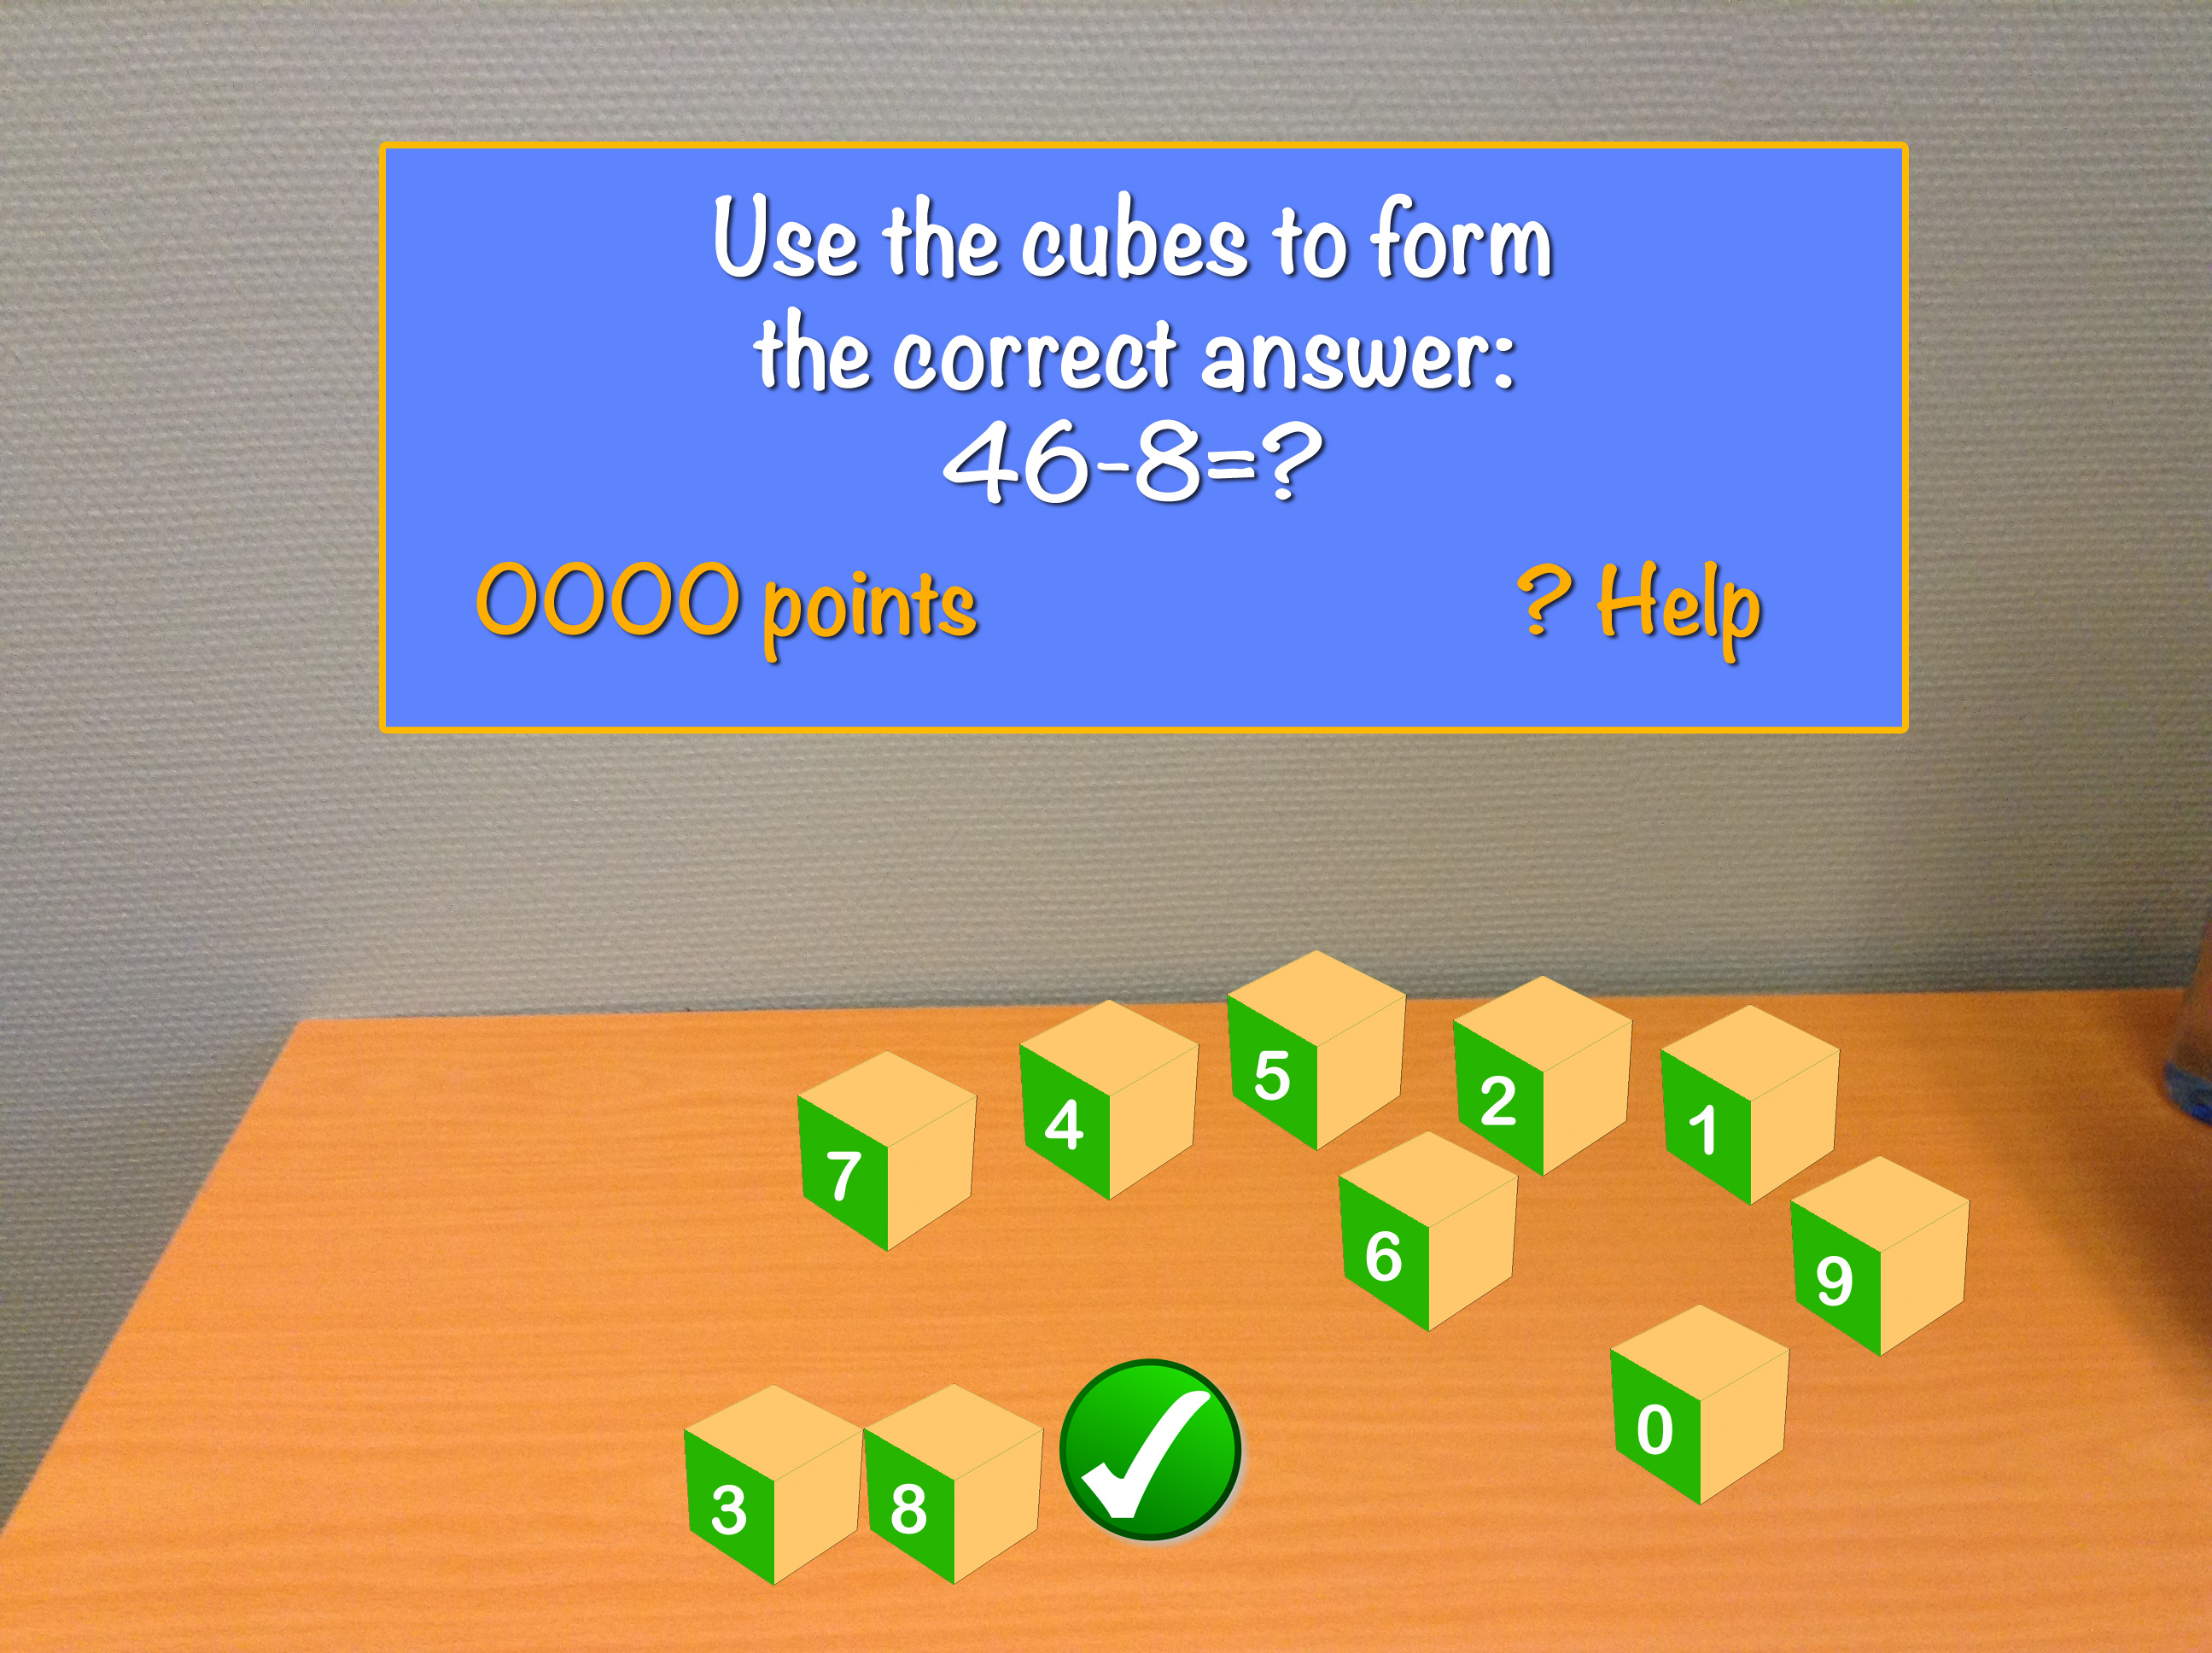
\includegraphics[width=0.9\textwidth]{images/Costas/game_mockup2(arithmetic2).jpg}
		\vspace{-10pt}
		\caption{Combining Numbers}
		\label{fig:Costas_combining_numbers}
	\end{minipage}%
	\label{fig:pair_games}
\end{figure}


\subsection{Total Sum}
\label{game:total_sum}

At the beginning of each level in this mini-game the cubes all have different numbers on them, both positive and negative numbers. The goal of the game is to combine cubes in a tower so that they together create the number on the top of the screen.
The level is over either when the sum is found or the time runs out.



\subsection{Combining Numbers}
	\label{game:combining_numbers}

When the game starts the player is shown a arithmetic calculation problem that the player have to solve. Using two cubes the player combines them to show the answer. For example '36 + 6' will results in the answer 42 so the player have to place the cube with the number four and two next to each other to create 42 (but not 24).
The level is over either when the answer is found or the time runs out.

\begin{figure}[h]
	\centering
	\begin{minipage}{.5\textwidth}
		\capstart
		\centering
		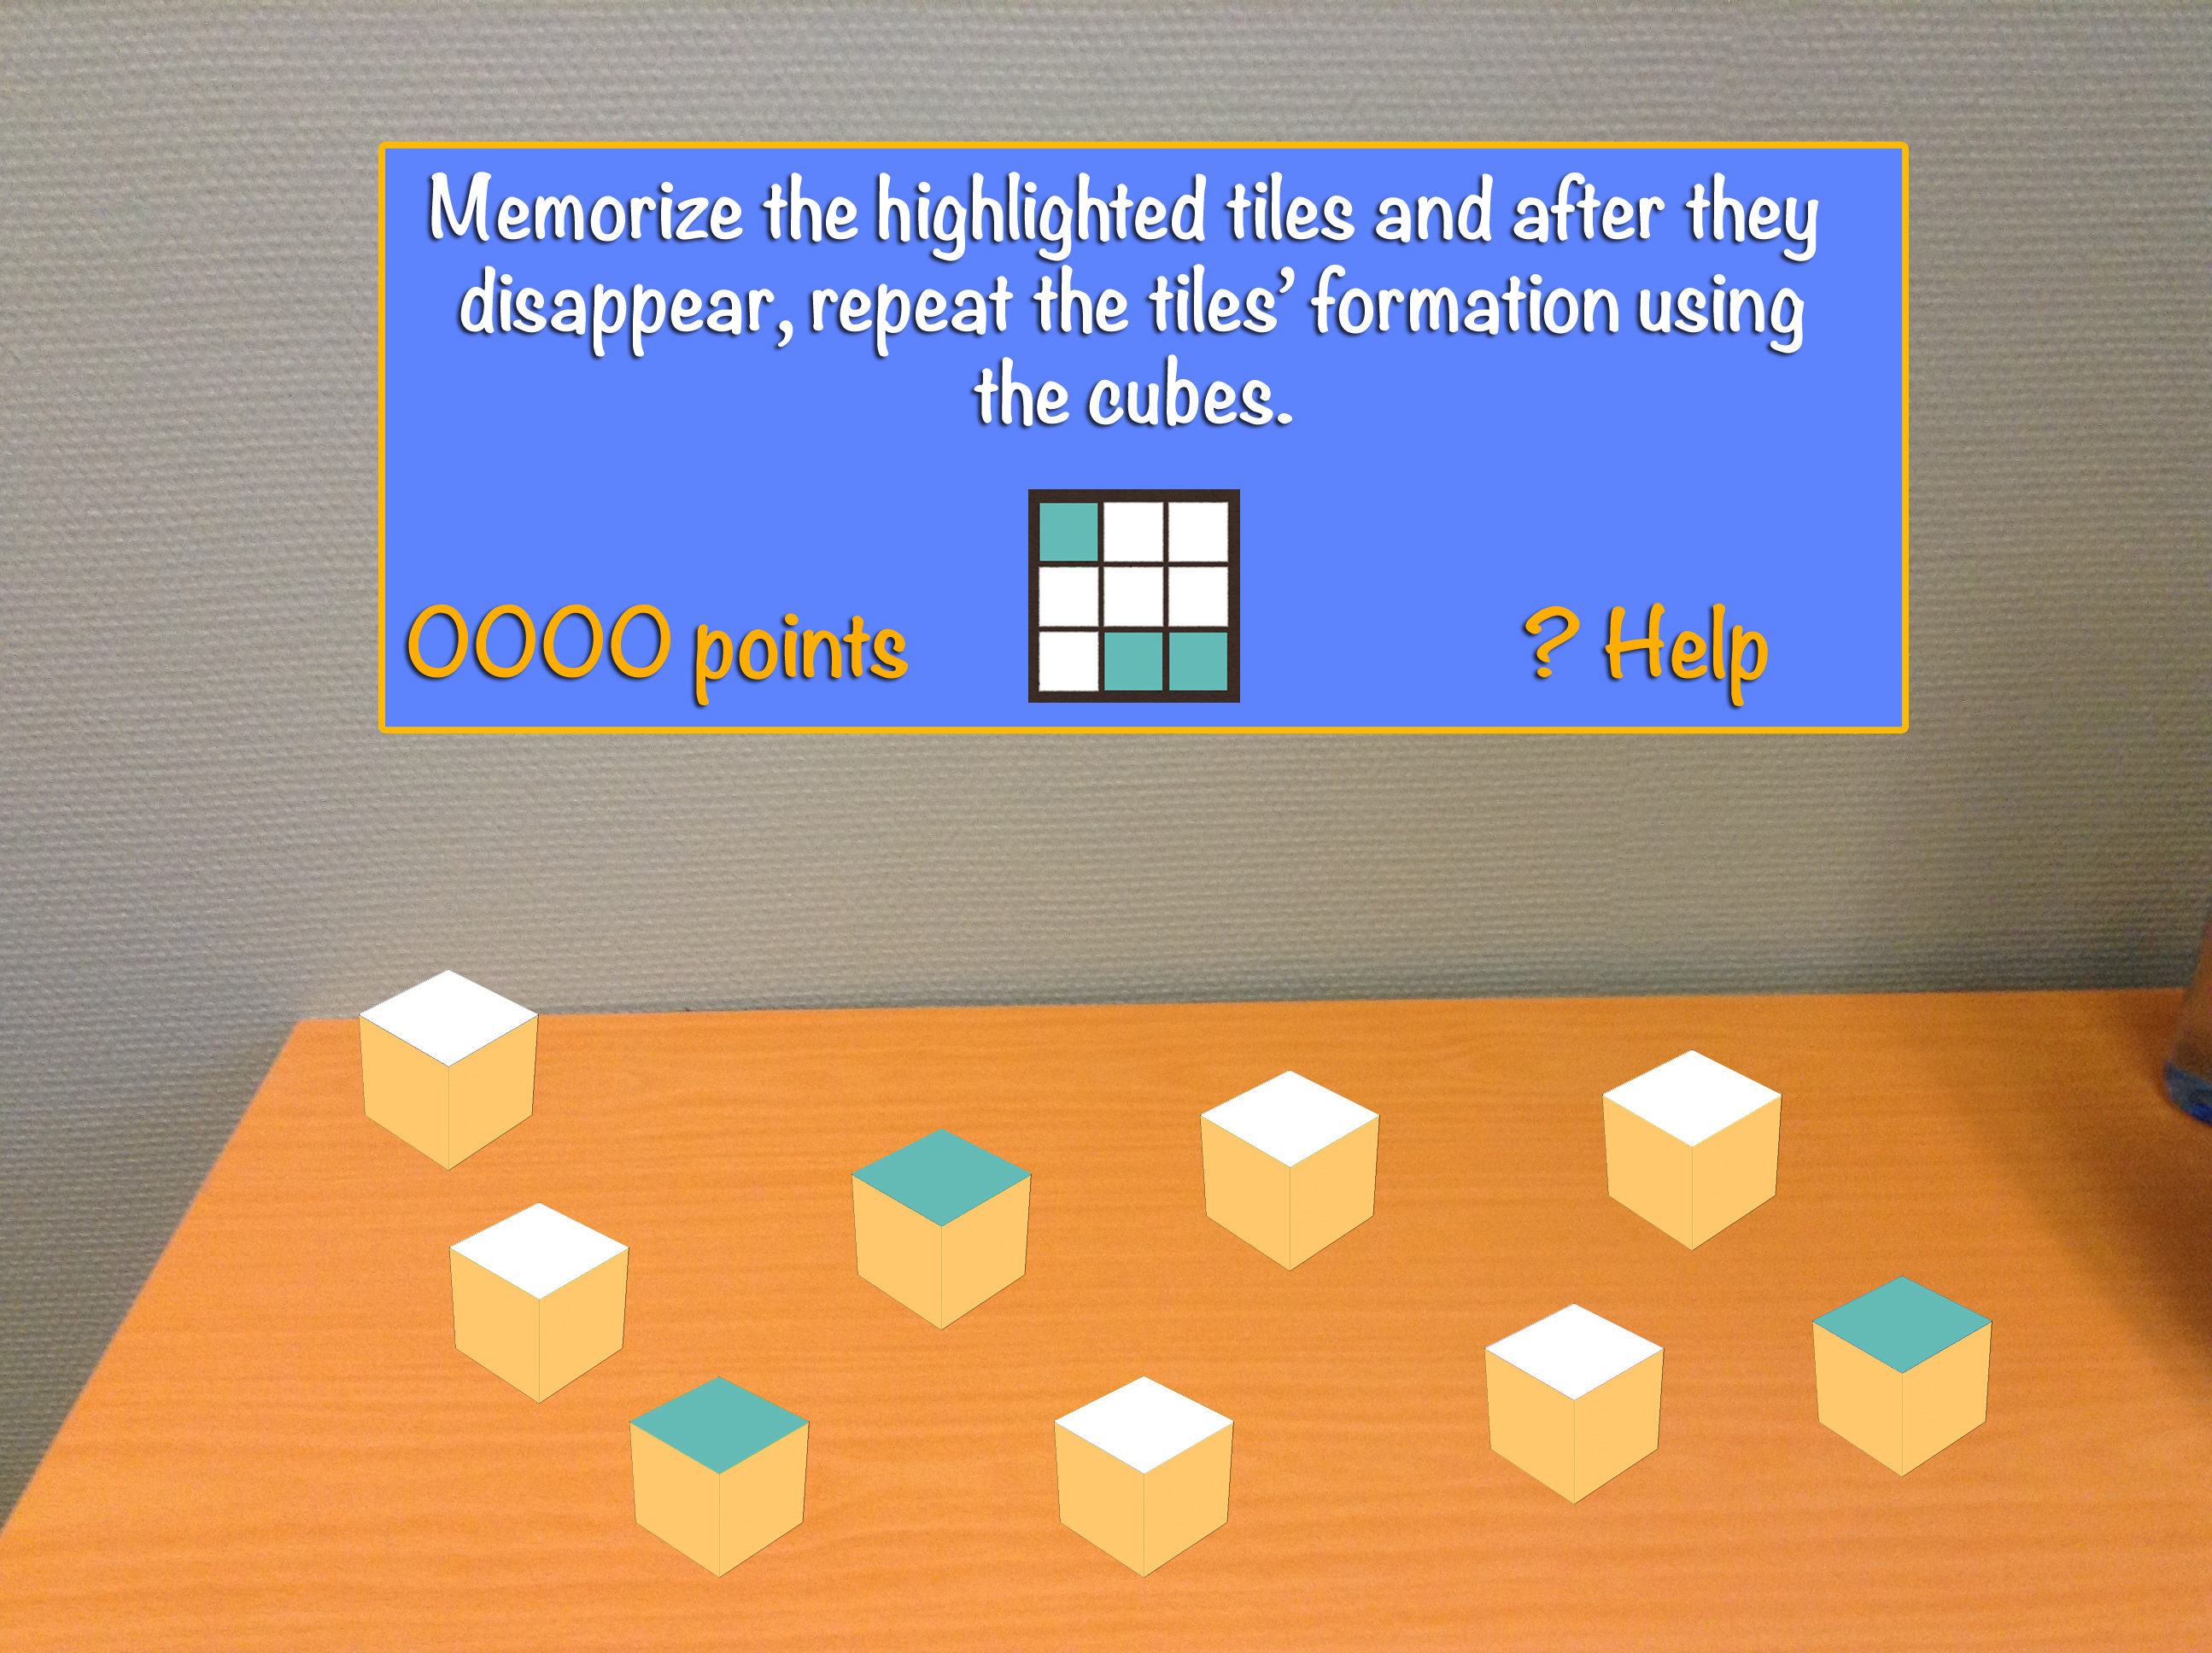
\includegraphics[width=0.9\textwidth]{images/Costas/game_mockup3(matrix).jpg}
		\vspace{-10pt}
		\caption{Pattern Memory}
		\label{fig:Costas_pattern_memory}
	\end{minipage}%
	\begin{minipage}{.5\textwidth}
		\capstart
		\centering
		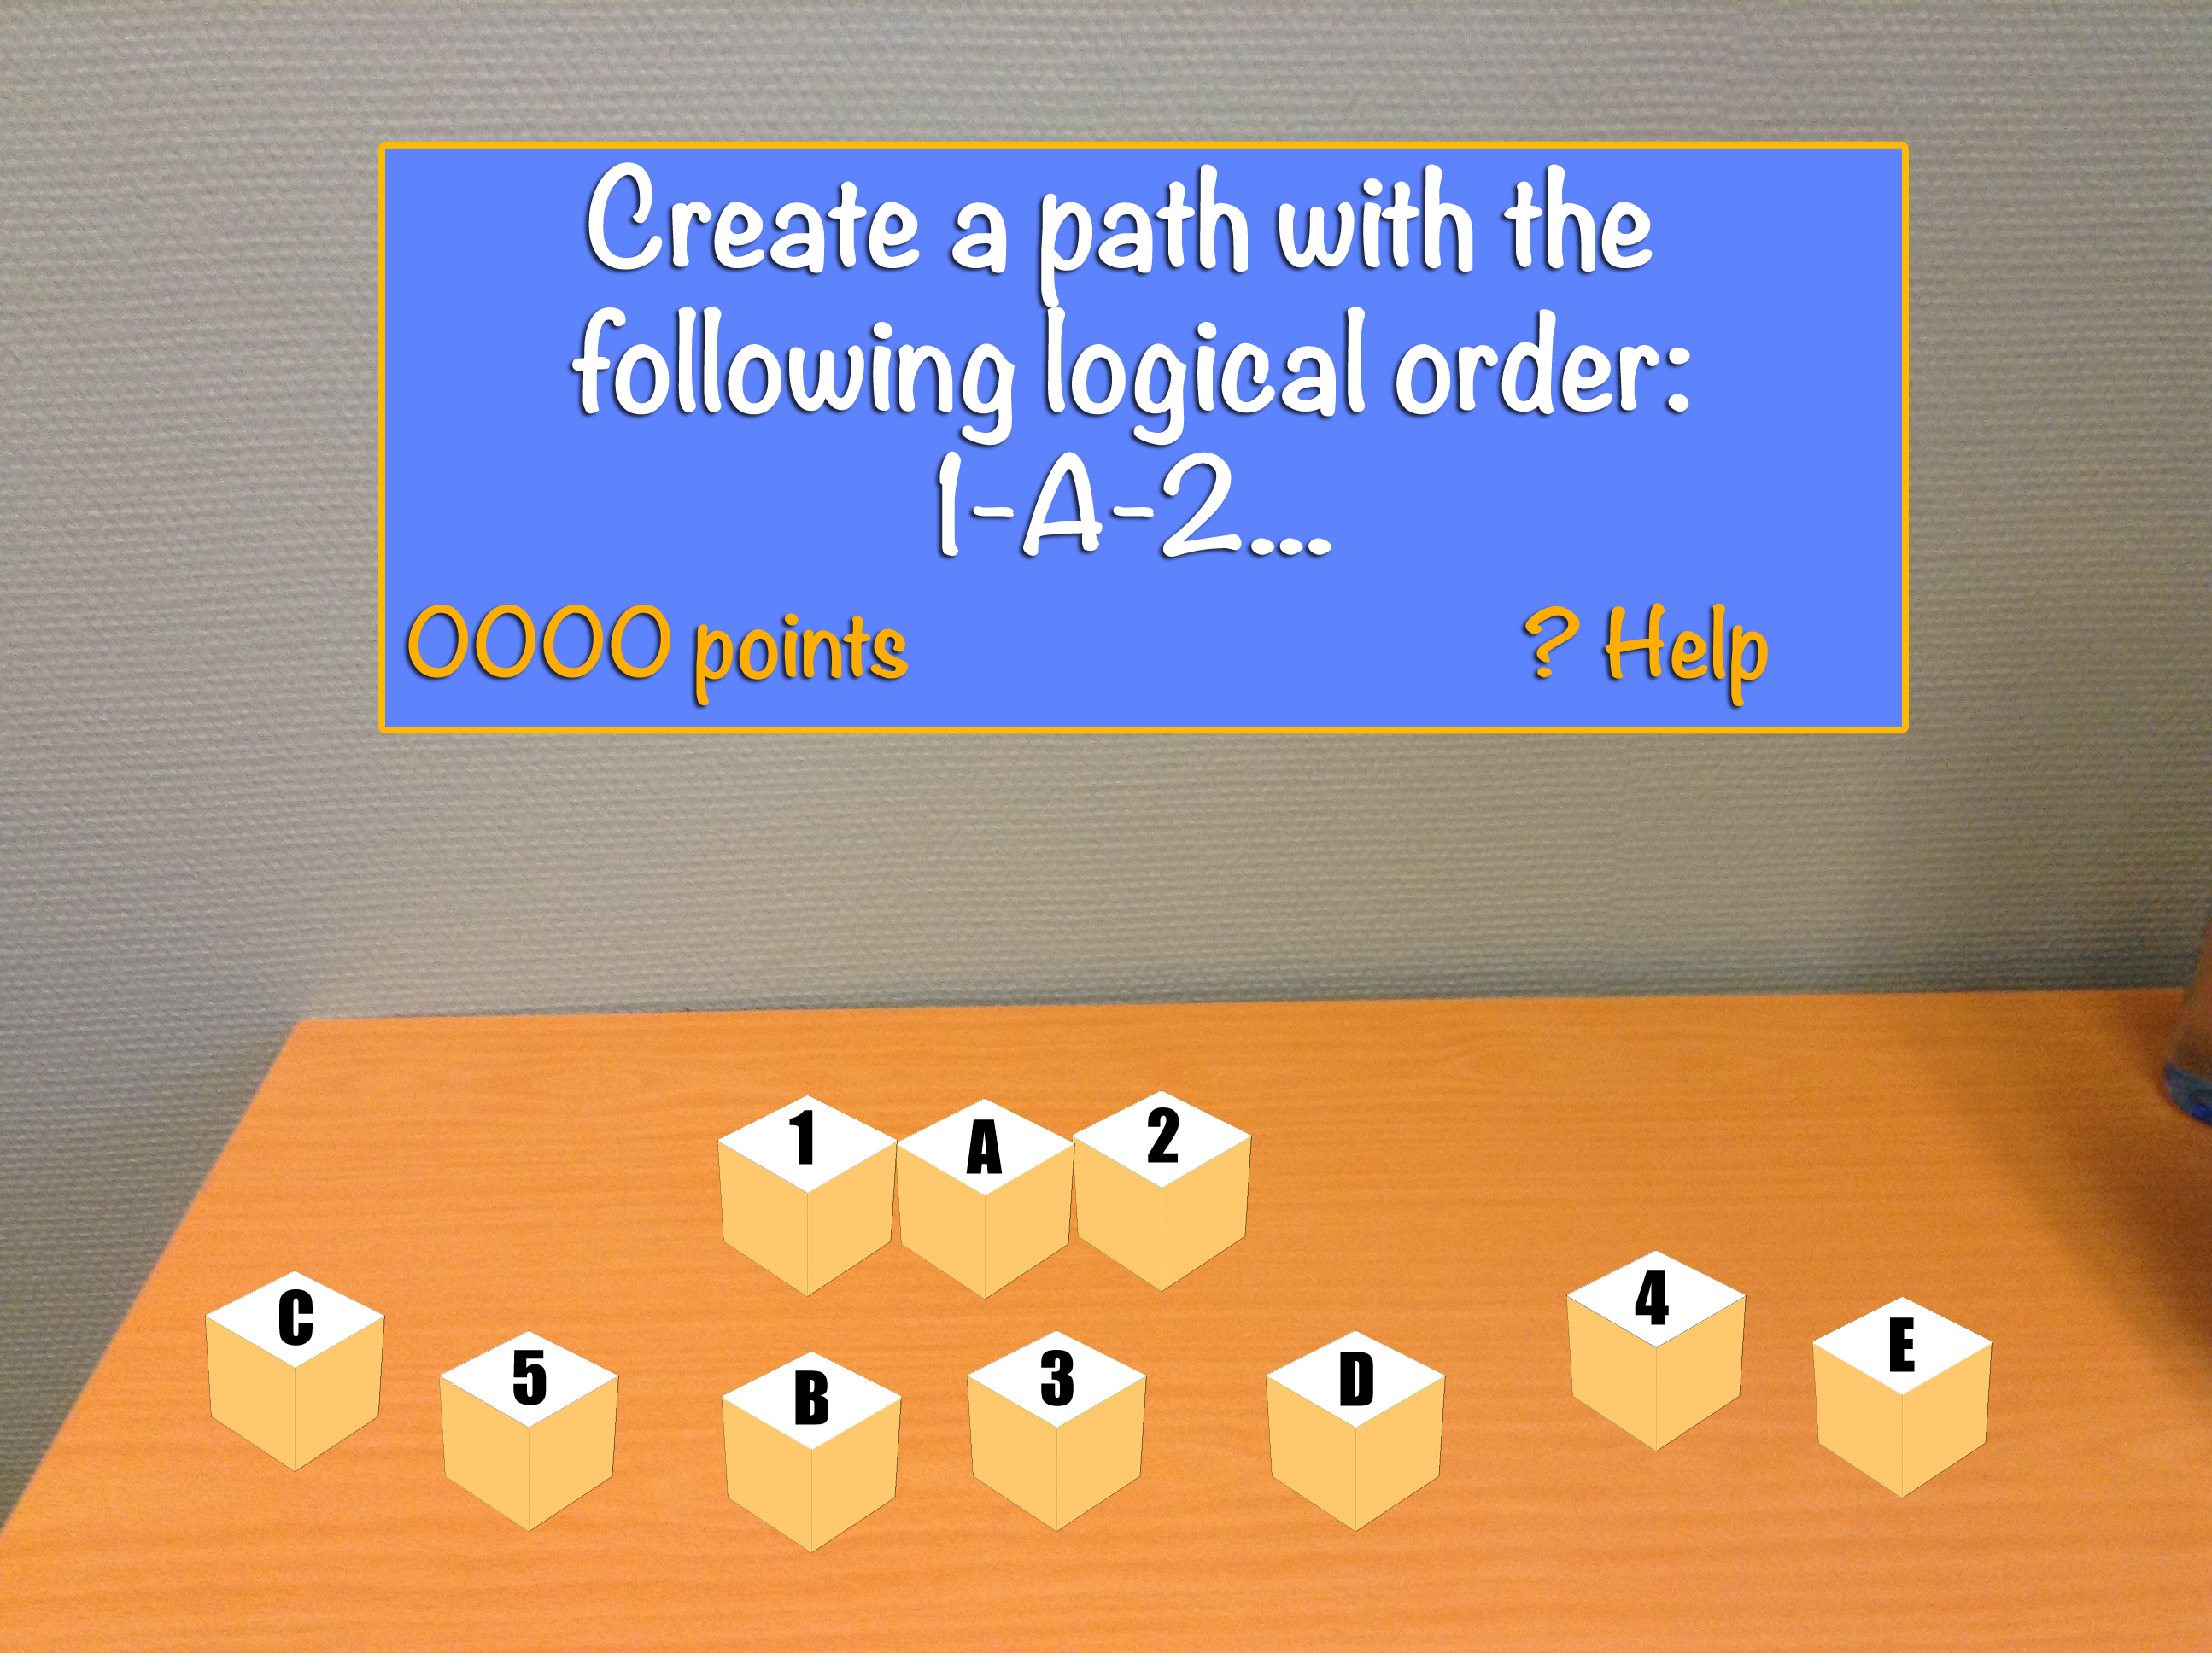
\includegraphics[width=0.9\textwidth]{images/Costas/game_mockup5(path).jpg}
		\vspace{-10pt}
		\caption{The Path}
		\label{fig:Costas_the_path}
	\end{minipage}%
\end{figure}


\subsection{Pattern Memory}
	\label{game:pattern_memory}

At the beginning of each level the player is shown a grid of nine cubes where the cubes can have two different colours, the goal of the game is to place the cubes in a grid making the same pattern as shown in the grid at the beginning of the level. The level is over either when the player have successfully recreated the grid pattern or the time runs out.


\subsection{The Path}
	\label{game:the_path}

Using the cubes the player have to make a logical path using all of the cubes. The five of the cubes have letters from A to E, and five have the numbers 1 to 5. The goal was then to make a line showing 1A2B3C4D5E. The game is over either when the path is completed or when the time runs out.


\begin{figure}[h]
	\centering
	\begin{minipage}{.5\textwidth}
		\capstart
		\centering
		\vspace{10pt}
		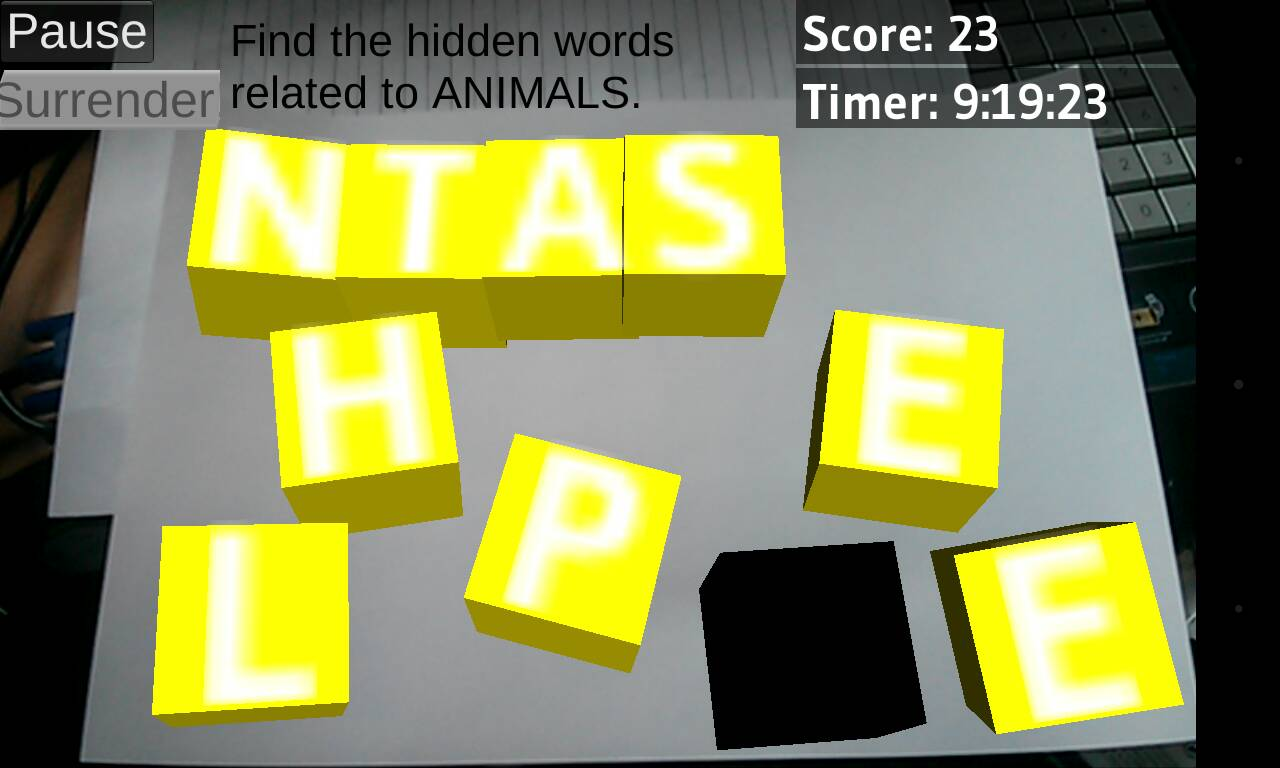
\includegraphics[width=0.9\textwidth]{images/Wo0ords_screenshot.jpg}
		\vspace{-10pt}
		\caption{Wo0ord Game}
		\label{fig:Costas_wo0ords}
	\end{minipage}%
\end{figure}


\subsection{Wo0ord Game}
	\label{game:wo0ord_game}
	
For this game the player is presented with a theme at the beginning of the stage, and using all the cubes which have letters on them combine them to make words related to the theme, the level is over when the player have either found 